% !TeX root = ./0Base.tex

\chapter{Results}\label{cha:results}

\section{Performance}

Graphs below (\ref{tab:resultsGet}, \ref{tab:resultsGetMany}, \ref{tab:resultsDelete}, \ref{tab:resultsPost} and \ref{tab:resultsPut}) show an average response time in miliseconds by number of concurrent \acrshort{vu}s from the tests mentioned in previous chapters. To better show the results of the tests, on vertical axis a logarithmic scale has been used, as Django had very long response times in comparison to other two frameworks. Under each graph there is a table with data used to draw the mentioned graphs - average response times rounded to second decimal place. As seen on the results, in cases with small amount concurrent requests Express.js application was the fastest. Starting from 32 \acrlong{vu}s for get requests, 128 for post and put requests and 512 for getMany ASP.NET Core has faster results. The trend line in all charts (except for delete tests, where ASP.NET is slower than express in all tests by from 8\% to 49\% depending on concurrency) shows that Express.js handles bigger loads worse than ASP.NET. In most tests Django stands out very far from the others, being even up to almost 17 times slower (for get tests with 8 concurrency) than the opponents. This framework surprised on getMany tests, where it was slower by only 15\% than the second best result - ASP.NET. 

\begin{figure}[H]
    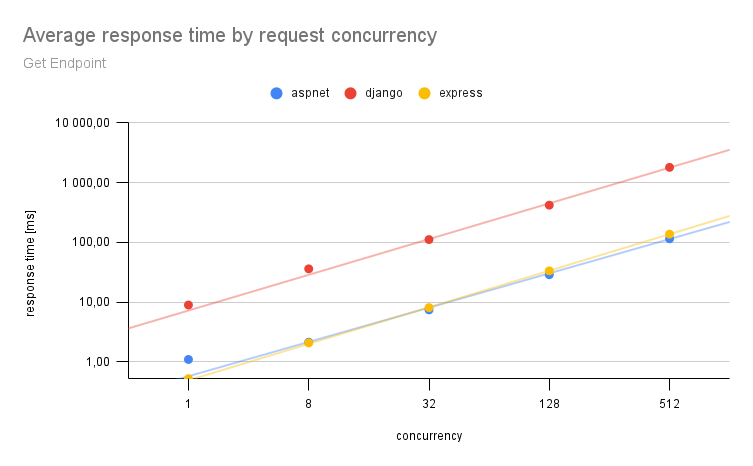
\includegraphics[width=\columnwidth]{figures/pictures/resultsGet.png}
    \caption{Average response time in get tests}
    \label{fig:resultsGet}
\end{figure}

\FloatBarrier
\begin{table}[!htp]\centering
    \caption{Average p(95) response time in tests}\label{tab:resultsGet}
    \scriptsize
    \begin{tabular}{lrrrrr}\toprule
        test & concurrency & aspnet & django   & express \\\midrule
        get  & 1           & 1.09   & 8.90     & 0.51    \\
        get  & 8           & 1.97   & 32.06    & 1.73    \\
        get  & 32          & 6.26   & 94.71    & 6.52    \\
        get  & 128         & 23.38  & 338.88   & 26.14   \\
        get  & 512         & 92.81  & 1,411.91 & 108.42  \\
        \bottomrule
    \end{tabular}
\end{table}
\FloatBarrier


\begin{figure}[H]
    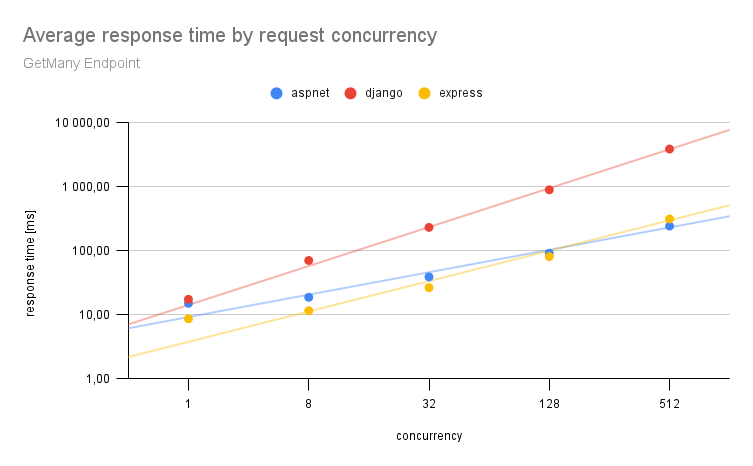
\includegraphics[width=\columnwidth]{figures/pictures/resultsGetMany.png}
    \caption{Average response time in getMany tests}
    \label{fig:resultsGetMany}
\end{figure}

\FloatBarrier
\begin{table}[!htp]\centering
    \caption{Average p(95) response time in tests}\label{tab:resultsGetMany}
    \scriptsize
    \begin{tabular}{lrrrrr}\toprule
        test    & concurrency & aspnet & django    & express \\\midrule
        getMany & 1           & 47.75  & 54.77     & 10.37   \\
        getMany & 8           & 42.03  & 267.56    & 11.72   \\
        getMany & 32          & 62.94  & 979.83    & 25.03   \\
        getMany & 128         & 112.69 & 3,897.61  & 69.38   \\
        getMany & 512         & 273.04 & 15,952.84 & 252.17  \\
        \bottomrule
    \end{tabular}
\end{table}
\FloatBarrier


\begin{figure}[H]
    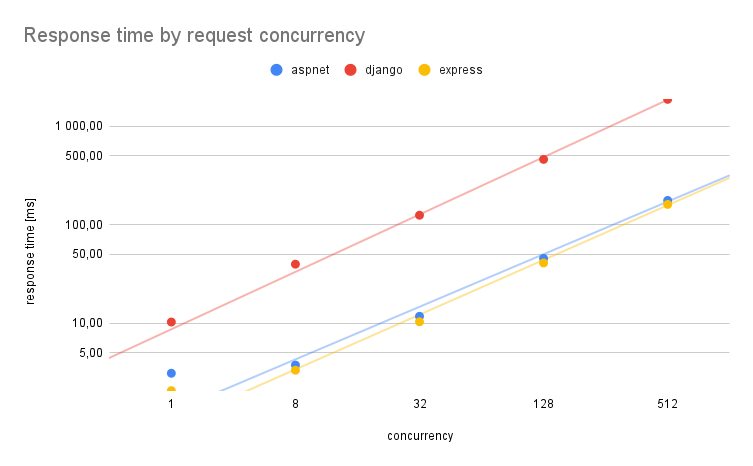
\includegraphics[width=\columnwidth]{figures/pictures/resultsDelete.png}
    \caption{Numeric results from delete tests}
    \label{fig:resultsDelete}
\end{figure}

\FloatBarrier
\begin{table}[!htp]\centering
    \caption{Average p(95) response time in tests}\label{tab:resultsDelete}
    \scriptsize
    \begin{tabular}{lrrrrr}\toprule
        test   & concurrency & aspnet & django   & express \\\midrule
        delete & 1           & 3.11   & 10.30    & 2.07    \\
        delete & 8           & 3.76   & 39.81    & 3.34    \\
        delete & 32          & 11.77  & 125.11   & 10.36   \\
        delete & 128         & 45.53  & 461.95   & 40.98   \\
        delete & 512         & 176.82 & 1,879.71 & 161.20  \\
        \bottomrule
    \end{tabular}
\end{table}
\FloatBarrier


\begin{figure}[H]
    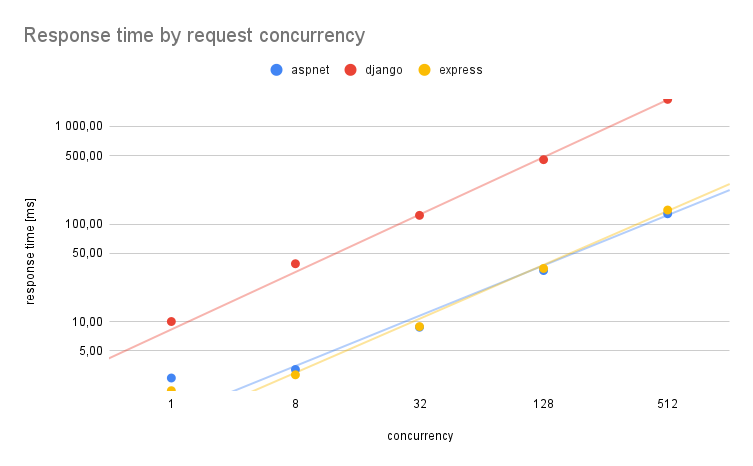
\includegraphics[width=\columnwidth]{figures/pictures/resultsPost.png}
    \caption{Numeric results from post tests}
    \label{fig:resultsPost}
\end{figure}

\FloatBarrier
\begin{table}[!htp]\centering
    \caption{Numeric results from post tests}\label{tab:resultsPost}
    \scriptsize
    \begin{tabular}{lrrrrr}\toprule
        test & concurrency & aspnet & django   & express \\\midrule
        post & 1           & 2.64   & 10.06    & 1.96    \\
        post & 8           & 3.29   & 45.23    & 3.02    \\
        post & 32          & 12.44  & 146.03   & 10.10   \\
        post & 128         & 38.54  & 564.70   & 40.40   \\
        post & 512         & 150.11 & 2,360.03 & 165.16  \\
        \bottomrule
    \end{tabular}
\end{table}
\FloatBarrier


\begin{figure}[H]
    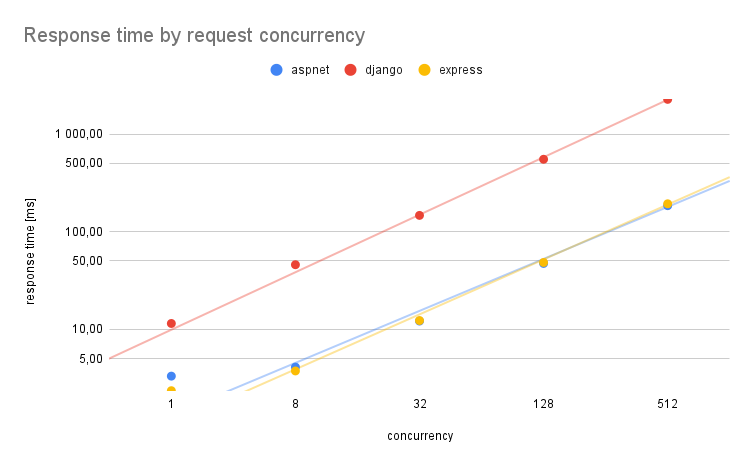
\includegraphics[width=\columnwidth]{figures/pictures/resultsPut.png}
    \caption{Numeric results from put tests}
    \label{fig:resultsPut}
\end{figure}

\FloatBarrier
\begin{table}[!htp]\centering
    \caption{Average p(95) response time in tests}\label{tab:resultsPut}
    \scriptsize
    \begin{tabular}{lrrrrr}\toprule
        test & concurrency & aspnet & django   & express \\\midrule
        put  & 1           & 3.30   & 11.44    & 2.34    \\
        put  & 8           & 4.08   & 45.78    & 3.73    \\
        put  & 32          & 12.10  & 146.66   & 12.25   \\
        put  & 128         & 47.18  & 551.59   & 48.27   \\
        put  & 512         & 184.42 & 2,268.39 & 192.83  \\
        \bottomrule
    \end{tabular}
\end{table}
\FloatBarrier


\section{Security}
\subsection{Security Misconfiguration}
\subsubsection{Django specific variables}
Django has one configuration file, generated automatically at the project creation. At the starting lines of settings.py a few important variables and comments are placed (listing \ref{lst:djangoSettings}).
\begin{lstlisting}[language=Python,caption={Fragment of unchanged newly generated Django settings file},breaklines=true,label={lst:djangoSettings}]
    # Quick-start development settings - unsuitable for production
    # See https://docs.djangoproject.com/en/3.1/howto/deployment/checklist/
    
    # SECURITY WARNING: keep the secret key used in production secret!
    SECRET_KEY = 'k!vv90$1&z+%fhv!+c^#1pfe_f&jim&tv7$yk%d9wspv=)#$x+'
    
    # SECURITY WARNING: don't run with debug turned on in production!
    DEBUG = True
    
    ALLOWED_HOSTS = []
\end{lstlisting}
.
As we can see, the creators of Django clearly want the developers to prevent some security vulnerabilities, by placing \lstinline{SECURITY WARNING} comments above two crucial variables - \lstinline{SECRET_KEY} and \lstinline{DEBUG}.
\lstinline{SECRET_KEY} is used in:
\begin{itemize}
    \item Generating session tokens
    \item Generating password reset tokens
    \item Ensuring that data passed from django forms is not changed
    \item Generating secret URLs for temporary access to a protected resource (for example a file)
    \item And any other cryptographic signing, unless a developer provides a different key
          % TODO ref https://docs.djangoproject.com/en/3.2/ref/settings/#secret-key 
          %  https://docs.djangoproject.com/en/3.2/topics/signing/
\end{itemize}.
All of them are very serious risks and should be avoided by any means. App created for this research is tiny does not have any serious logic other than working on a database model, so cryptographic signing is not used at all. For any commercial applications leaking this variable could cause a lot of harm.
The second risky variable - \lstinline{DEBUG} - is responsible for turning on and off a debug mode. When set to True, whenever an error happens Django will display a detailed traceback, including parts of the applications source code and environment variables (such as Django settings).
Django developers thought about it being a little secure in case of accidental leakage by excluding from the message variables containing the following strings:
\begin{itemize}
    \item 'API'
    \item 'KEY'
    \item 'PASS'
    \item 'SECRET'
    \item 'SIGNATURE'
    \item 'TOKEN'
\end{itemize}
% TODO show a screen where if(id === 10): admin = True 
% coś jak to https://www.troyhunt.com/content/images/2016/02/848847image11.png

Third important variable that cannot be forgotten is \lstinline{ALLOWED_HOSTS} (without \lstinline{SECURITY WARNING} comment, as it is set to an empty array by default). This variable is meant to be a list of strings presenting host names that Django can send responses to. If a given host is not on the list and tries to request a resource, response with status 400 is sent immediately. When \lstinline{DEBUG} is set to True and this variable is empty, the only way to get response from the app is by requesting localhost.

To help the developers, Django offers a command \lstinline{python3 manage.py check --deploy} command.
\begin{lstlisting}[keywordstyle=\color{black},caption={Warnings shown by Django check deploy command on fresh project},breaklines=true,label={lst:djangoCheckDeploy}]
    > python3 manage.py check --deploy
    System check identified some issues:
    
    WARNINGS:
    ?: (security.W004) You have not set a value for the SECURE_HSTS_SECONDS setting. If your entire site is served only over SSL, you may want to consider setting a value and enabling HTTP Strict Transport Security. Be sure to read the documentation first; enabling HSTS carelessly can cause serious, irreversible problems.
    ?: (security.W008) Your SECURE_SSL_REDIRECT setting is not set to True. Unless your site should be available over both SSL and non-SSL connections, you may want to either set this setting True or configure a load balancer or reverse-proxy server to redirect all connections to HTTPS.
    ?: (security.W012) SESSION_COOKIE_SECURE is not set to True. Using a secure-only session cookie makes it more difficult for network traffic sniffers to hijack user sessions.
    ?: (security.W016) You have 'django.middleware.csrf.CsrfViewMiddleware' in your MIDDLEWARE, but you have not set CSRF_COOKIE_SECURE to True. Using a secure-only CSRF cookie makes it more difficult for network traffic sniffers to steal the CSRF token.
    ?: (security.W018) You should not have DEBUG set to True in deployment.
    ?: (security.W020) ALLOWED_HOSTS must not be empty in deployment.
    
    System check identified 6 issues (0 silenced).
\end{lstlisting}

% https://docs.djangoproject.com/en/3.2/howto/deployment/checklist/
% python3 manage.py check --deploy
% https://hdivsecurity.com/owasp-security-misconfiguration
\subsubsection{ASP.NET}

Just like Django, ASP.NET can leak sensitive data placed in code with its default error handling.

% TODO prepare a screen and write about it https://www.troyhunt.com/owasp-top-10-for-net-developers-part-6/

\subsubsection{Common}
\begin{itemize}
    \item Use newest versions
    % https://snyk.io/vuln/
    \item Don't configure to run as root
    \item limit request body size
    \item tls/ssl
    % https://nodegoat.herokuapp.com/tutorial/a5
\end{itemize}

\subsection{Injection}
\subsubsection{Django}
\subsubsection{ASP.NET}
\subsubsection{Express.js}
% DJANGO
% https://hdivsecurity.com/sql-injection-prevention
% https://docs.djangoproject.com/en/3.2/topics/security/#sql-injection-protection
% Injections can be done using inserting raw() queries
\subsection{Insufficient Logging}
\subsubsection{Django}
\subsubsection{ASP.NET}
\subsubsection{Express.js}
% DJANGO
% https://docs.djangoproject.com/en/3.0/topics/logging/
% https://pypi.org/project/django-automated-logging/
% https://pypi.org/project/django-log-viewer/
% When your application has insufficient logging and monitoring, attacks and suspicious activity can go unnoticed. By default, Django uses the Python native logging module for system logging. 
% django.security.* logging messages.

% ASPNET
% https://www.infoq.com/presentations/owasp-top-10-vulnerabilities-2017/
